\section{Implementation}
\label{section:implementation}
Using Hadoop v1.2.1, we were able to build and run a wordcount job
on both a single-node setup and a distributed two-node setup. Once
we had achieved this, we began instrumenting the code with extra,
custom logging to better understand how Hadoop works. Using the
logging and growing understanding of the Hadoop code base, we were
able to identify a couple key code insertion/modification points.

\subsection{Modifying Split Sizes}
One of the fundamental tasks we set out to achieve was to modify the
sizes of input splits. We found that the \texttt{InputSplit.getSplits()}
method, defined in \texttt{FileInputFormat.java} offered the cleanest
point for us to modify the splits. We opted for a contrived proof of
concept implementation, where we treated the job as static (by running
the same job repeatedly on the same machines) and forcing half of the
splits to be large. Our modification aims to be unobtrusive to Hadoop's
normal split algorithms by simply using a \texttt{minSize} to force larger
splits to occur. The code to do so is shown in \ref{fig:getSplitsCode}.

\begin{figure}[ht!]
\centering
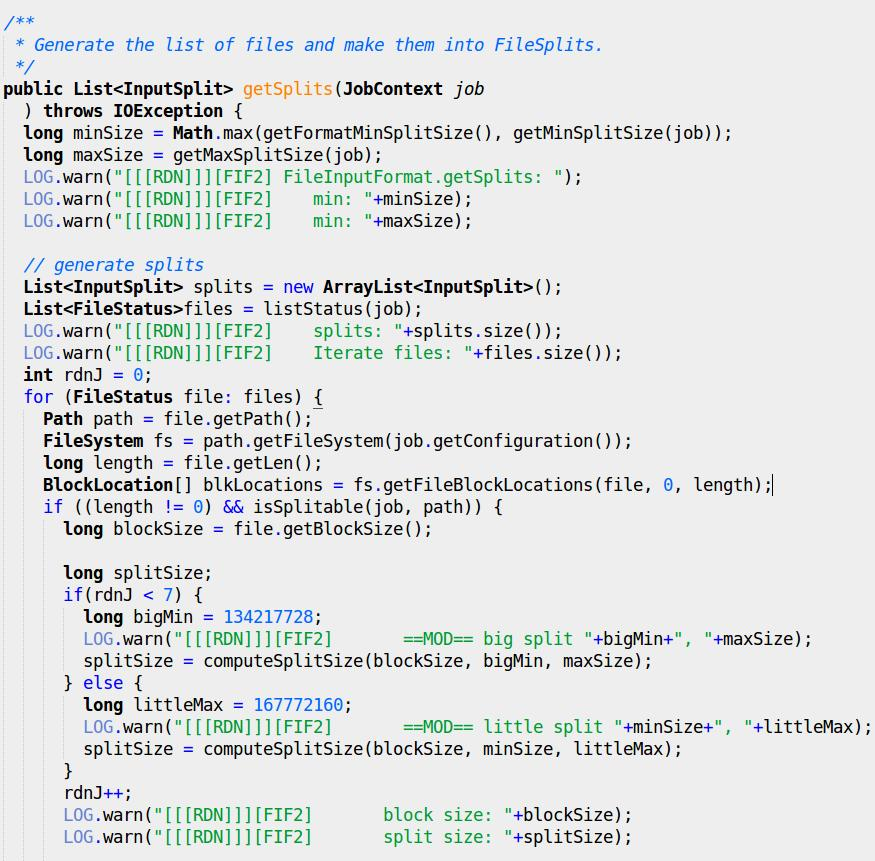
\includegraphics[width=90mm]{getSplitsCode.jpg}
\caption{Code coercing modified split sizes}
\label{fig:getSplitsCode}
\end{figure}

We then used log statements to confirm the splits were modified successfully.
An example of these log statements is shown in \ref{fig:getSplitsLog}.

\begin{figure}[ht!]
\centering
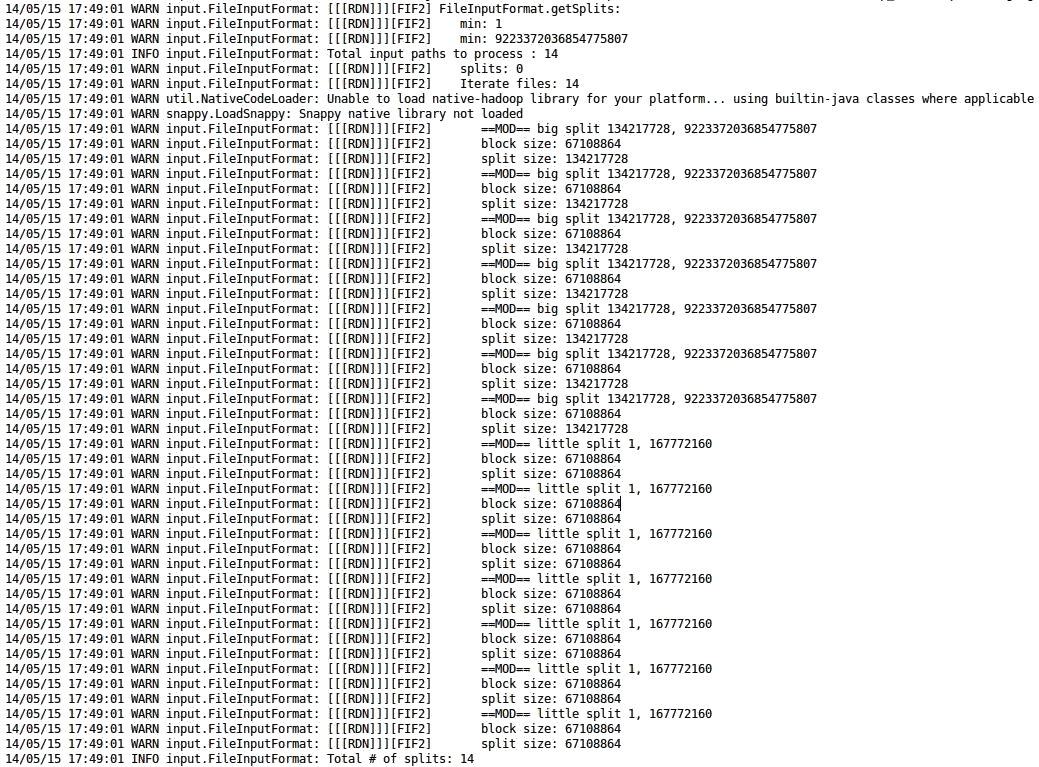
\includegraphics[width=90mm]{getSplitsLog.jpg}
\caption{Logs showing modified split sizes in a wordcount job}
\label{fig:getSplitsLog}
\end{figure}

\subsection{Classifying Host Capabilities}
Simply creating different size input splits is not sufficient for increasing
performance without associating which node or classification of node should
get which size split. There are several ways in which this can be done.
The simplest way to tie performance information to nodes in the Hadoop
environment would be to create a file in the \texttt{conf/} directory with
this information, and modifying the
\texttt{JobConf} class to parse in any new properties we define. A rudimentary
method would be to define two or more static input split sizes and two or more
classifications of nodes, identifying which nodes belong to which category.
We would then
use this configuration to determine how many and of what size splits to make
in \texttt{getSplits}, and then which nodes should get which sized splits
in the \texttt{TaskScheduler}. The \texttt{TaskScheduler} uses the
\texttt{TaskTrackerStatus} to get information about the node it is currently
assigning tasks to. This class could be modified to contain the classification
information about that node and then it could determine which input split size
to give it. A more dynamic solution would be to have each node report current
performance metrics in its \texttt{heartbeat} to the JobTracker. This metric
would then determine what input split size to give it. This method would also be
somewhat sensitive to degraded performance on that node caused by interference
from third party VMs running on the same hardware.
